\documentclass[a4paper, openany]{memoir}

\usepackage[utf8]{inputenc}
\usepackage[T1]{fontenc} 
\usepackage[english]{babel}
\usepackage{fancyhdr}
\usepackage{float}
\usepackage{amsmath}
\usepackage{amsthm}
\usepackage{amssymb}
\usepackage[bookmarksopen=true,bookmarksopenlevel=2]{hyperref}
\usepackage{tikz}
\usepackage{indentfirst}
\usepackage{listings}

\definecolor{codegreen}{rgb}{0,0.6,0}
\definecolor{codegray}{rgb}{0.5,0.5,0.5}
\definecolor{codepurple}{rgb}{0.58,0,0.82}
\definecolor{backcolour}{rgb}{0.95,0.95,0.92}

\lstdefinestyle{thestyle}{
    backgroundcolor=\color{backcolour},
    basicstyle=\ttfamily\footnotesize,
    keywordstyle=\color{red!80}\bfseries,
    ndkeywordstyle=\color{blue!80}\bfseries,
    identifierstyle=\color{black},
    commentstyle=\color{codegreen},
    stringstyle=\color{codepurple},
    breakatwhitespace=false,
    breaklines=true,
    captionpos=b,
    keepspaces=true,
    numberstyle=\tiny\color{codegray},
    numbers=left,
    numbersep=2pt,
    showspaces=false,
    showstringspaces=false,
    showtabs=false,          
    tabsize=2
}

\lstdefinelanguage{calc}{ 
    keywords={set, put},
    ndkeywords={},
    sensitive=true,
    comment=[l]{//},
    morecomment=[s]{/*}{*/},
    morestring=[b]',
    morestring=[b]"
}

\lstset{style=thestyle}

\pagestyle{fancy}
\fancyhf{}
\fancyhead[LE]{\leftmark}
\fancyhead[RO]{\rightmark}
\fancyhead[RE, LO]{PL}
\fancyfoot[LE, RO]{\thepage}
\fancyfoot[RE, LO]{Pete Gautam}

\usetikzlibrary{shapes}

\renewcommand{\headrulewidth}{1.5pt}

\chapterstyle{thatcher}

\begin{document}
\chapter{Syntax, values and types}
\section{Syntax}
The syntax of a programming language (PL) is concerned with the form of a program. It considers how expressions, commands, declarations and other constructs are arranged to form a well-formed program. When we learn a new PL, we start by learning its syntax. Note that the syntax must be specified; examples are not enough to show the generality of the PL's syntax. To see this, consider the following code:
\begin{verbatim}
if n > 0: write (n)
\end{verbatim}
Although the example illustrates a way we can use an if-statement, it does not tell us all the possible ways we can use the if-statement. In particular,
\begin{itemize}
    \item within the \texttt{if} block, can we just have one command or multiple commands?
    \item within the \texttt{write} function, can we just make use of a variable or use any sort of expression?
\end{itemize}

\subsection{Formal specification of syntax}
There are two ways to specify the syntax- informal and formal specification. An informal specification is expressed in a natural language (e.g. English), while a formal specification is expressed in a precise notation. 

Formal specifications are more precise, usually more concise, while informal specifications tend to be ambiguous, inconsistent or incomplete. However, formal specifications are only accessible to those who are familiar with the notation, and is often difficult to use in practice.

We will illustrate the two types of specification with a while loop in a C-like language.
\begin{itemize}
    \item Informal specification: A while-command consists of \texttt{while}, followed by an expression enclosed in parentheses, followed by a sequential command. A sequential command consists of a sequence of one or more commands, enclosed by `\texttt{\{}' and `\texttt{\}}'.
    \item Formal specification, using EBNF:
    \begin{align*}
        \textit{while-command} =& \text{ `}\texttt{while}\text{' }  ( \textit{ expression } )  \textit{ sequential-command} \\
        \textit{sequential-command} =&  \text{ `}\texttt{\{}\text{' } \textit{command}^+ \text{ `}\texttt{\}}\text{'}
    \end{align*}
\end{itemize}

There are 3 ways we can specify the syntax of a PL formally:
\begin{itemize}
    \item Regular expression (RE) is good for specifying syntax of lexical elements of programs (e.g. identifiers, literals and comments).
    \item Backus Naur Form (BNF) is good for specifying syntax of larger and nested program constructs (e.g. expressions, commands and declarations).
    \item Extended Backus Naur Form (EBNF) combines RE and BNF, and are good in almost all the cases.
\end{itemize}

We will illustrate syntax using the PL Calc. It is a very simple calculator language, with:
\begin{itemize}
    \item variables named \texttt{a}, \texttt{b}, ..., \texttt{z} (i.e. lowercase Roman characters).
    \item expressions consisting of variables numerals and arithmetic operators.
    \item assignment (\texttt{set}) and output (\texttt{put}) commands.
\end{itemize}
The following is a Calc program:
\begin{lstlisting}[language=calc]
set x = 13
set y = x * (x + 1)
put x
put y / 2
\end{lstlisting}

\subsubsection{Regular expressions}
A RE is a type of pattern. That is, every RE matches a set of (possibly infinite) strings. We can use REs for a variety of applications:
\begin{itemize}
    \item specifying a pattern of strings to be searched for in a text.
    \item specifying a pattern of filenames to be searched for in a file system.
    \item specifying the syntax of a PL's lexical elements.
\end{itemize}
We will look at some examples of REs:
\begin{itemize}
    \item \texttt{M(r|rs|iss)} matches \texttt{Mr}, \texttt{Mrs} and \texttt{Miss}.
    \item $\texttt{b(an)}^{\texttt{*}}\texttt{a}$ matches \texttt{ba}, \texttt{bana}, \texttt{banana}, \texttt{bananana}, and so on.
    \item $\texttt{(x|abc)}^{\texttt{*}}$ matches \texttt{x}, \texttt{abc}, \texttt{xx}, \texttt{xabc}, \texttt{abcx}, and so on.
\end{itemize}
The following are the basic RE notations:
\begin{itemize}
    \item a literal \texttt{xyz} matches the literal \texttt{xyz} itself.
    \item $\texttt{RE}_1|\texttt{RE}_2$ matches a string that matches either the regular expression $\texttt{RE}_1$ or the regular expression $\texttt{RE}_2$.
    \item $\texttt{RE}_1 \ \texttt{RE}_2$ matches a string that matches the regular expression $\texttt{RE}_1$ concatenated with a string that matches the regular expression $\texttt{RE}_2$.
    \item $\texttt{RE}^{\texttt{*}}$ matches a string that is a concatenation of zero of more strings that match the regular expression \texttt{RE}.
    \item \texttt{(RE)} matches any string that matches the regular expression \texttt{RE} (and is used for grouping and precedence).
\end{itemize}
There are two further RE notations:
\begin{itemize}
    \item $\texttt{RE}^?$ matches either the empty string or a string that matches the regular expression \texttt{RE}. Its basic RE notation is $\texttt{RE}|\epsilon$.
    \item $\texttt{RE}^{\texttt{+}}$ matches a string that is a concatenation of one or more strings that match the regular expression \texttt{RE}. Its basic RE notation is $\texttt{RE} \ \texttt{RE}^{\texttt{*}}$.
\end{itemize}

In terms of Calc, we can use a RE to represent the possible identifiers. It is
\[\texttt{a}|\texttt{b}|\dots|\texttt{z}.\]
We can also use REs for numeral, which consist of one or more decimal digits, e.g. \texttt{5}, \texttt{12}, \texttt{20}. Its RE is
\[(\texttt{0}|\texttt{1}|\dots|\texttt{9})^{\texttt{+}}.\]
If we have a PL where an identifier consists of a sequence of one or more upper-case letters and digits, starting with a letter, then the syntax is given by the following RE
\[(\texttt{a}|\texttt{b}|\dots|\texttt{z}) (\texttt{a}|\texttt{b}|\dots|\texttt{z}|\texttt{0}|\texttt{1}|\dots|\texttt{9})^{\texttt{*}}.\]

REs are used everywhere. For instance, the Unix shell scripting language uses an ad hoc pattern-matching notation in which:
\begin{itemize}
    \item \texttt{[...]} matches any one of the enclosed characters;
    \item $\texttt{?}$ matches any single character;
    \item \texttt{*} matches any string of 0 or more characters.
\end{itemize}
This is a restricted variant of the RE notation since it lacks choice $\texttt{RE}_1|\texttt{RE}_2$ and the star $\texttt{RE}^{\texttt{*}}$ in their general form. Some example commands are:
\begin{itemize}
    \item \texttt{print bat.[chp]}, which prints files named either \texttt{bat.c}, \texttt{bat.h} or \texttt{bat.p}
    \item \texttt{print bat.?}, which prints all files whose names are \texttt{bat.}, followed by any single character
    \item \texttt{print *.c}, which prints all files whose names end with \texttt{.c}
\end{itemize}

Also, the Unix utility \texttt{egrep} uses the full pattern-matching notation, in which the following have their usual meanings: $\texttt{RE}_1|\texttt{RE}_2$,  $\texttt{RE*}$, $\texttt{RE+}$, $\texttt{RE?}$. It also provides extensions such as:
\begin{itemize}
    \item \texttt{[...]} which matches any of the enclosed characters and
    \item \texttt{.} which matches any single character.
\end{itemize}
Some example commands are given below:
\begin{itemize}
    \item \texttt{egrep `b[aei]t' file}, which finds all lines in \texttt{file} that contain \texttt{bat}, \texttt{bet} and \texttt{bit}.
    \item \texttt{egrep `b.t' file}, which finds all lines in \texttt{file} that contain \texttt{b}, followed by any character, and then \texttt{t}.
    \item \texttt{egrep `b(an)*a' file}, which finds all lines in \texttt{file} that contain \texttt{b}, followed by 0 or more occurrences of \texttt{an}, followed by \texttt{a}.
\end{itemize}

Moreover, some Java classes also use the full pattern-matching notation, with the same extension as \texttt{egrep}. An example is given below.
\begin{lstlisting}[language=java]
String s;
if (s.matches("b.t")) {
    // code
}
if (s.matches("b[aei]]t")) {
    // code
}
if (s.matches("b(ab)*a")) {
    // code
}
\end{lstlisting}

\subsection{BNF}
Although RE have many applications, they are not powerful enough to express the syntax of nested/embedded phrases. For example,
\begin{itemize}
    \item the nested expression \texttt{n * (n + 1)} and
    \item the nested loop 
\begin{lstlisting}[language=java]
while (r > 0) {
    m = n;
    n = r;
}
\end{lstlisting}
\end{itemize}
cannot be expressed using REs. 

To specify the syntax of nested phrases such as expressions and commands, we need a context-free grammar. The grammar of a language is a set of rules specifying how the phrases of that language are formed. Each rule specifies how each phrase may be formed from symbols, such as words and punctuation, and simpler phrases.

We are familiar with grammar in English. For example, the following sentences in English are valid: \texttt{I smell a rat} and \texttt{the cat sees me}. We refer to the symbols \texttt{a}, \texttt{cat}, \texttt{I}, etc. by terminal symbols. We denote these words using grammatical words, such as \textit{sentence}, \textit{subject}, \textit{object}, etc. These are non-terminal symbols.

To produce sentences in English, we have production rules, some of which are given below:
\begin{align*}
    \textit{sentence } =& \textit{ subject} \ \ \textit{verb} \ \ \textit{object} \text{ `}\texttt{.}\text{'} \\
    \textit{subject } =& \text{ `}\texttt{I}\text{' } | \text{ `}\texttt{a}\text{' } \textit{noun } | \text{ `}\texttt{the}\text{' } \textit{noun} \\
    \textit{object } =& \text{ `}\texttt{me}\text{' } | \text{ `}\texttt{a}\text{' } \textit{noun } | \text{ `}\texttt{the}\text{' } \textit{noun} \\
    \textit{noun } =& \text{ `}\texttt{cat}\text{' } | \text{ `}\texttt{mat}\text{' } | \text{ `}\texttt{rat}\text{'} \\
    \textit{verb } =&  \text{ `}\texttt{see}\text{' } | \text{ `}\texttt{sees}\text{' } | \text{ `}\texttt{smell}\text{' } | \text{ `}\texttt{smells}\text{'}
\end{align*}
We use equality to show precisely what we mean, e.g. by a sentence. We use the pipe | to denote different possible values, e.g. a noun can be \texttt{cat}, \texttt{mat} or \texttt{rat}. Using the production rules, we can describe how the sentence \texttt{I smell a rat} is structured, using a syntax tree.
\begin{figure}[H]
    \centering
    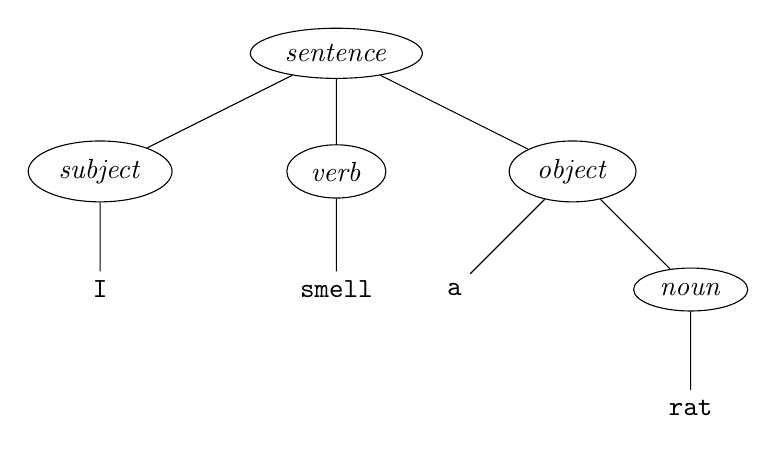
\begin{tikzpicture}[
    level 1/.style={sibling distance=3cm}
    ]
        \node[ellipse, draw] {\textit{sentence}}
        child {
            node[ellipse, draw] {\textit{subject}}
            child {
                node {\texttt{I}}
            }
        }
        child {
            node[ellipse, draw] {\textit{verb}}
            child {
                node {\texttt{smell}}
            }
        }
        child {
            node[ellipse, draw] {\textit{object}}
            child {
                node {\texttt{a}}
            }
            child {
                node[ellipse, draw] {\textit{noun}}
                child {
                    node {\texttt{rat}}
                }
            }
        };
    \end{tikzpicture}
    \caption{The syntax tree for \texttt{I smell a rat}}
\end{figure}
\noindent The non-terminal symbols are circled. Note that the terminal symbols are precisely composed of the leaves. Reading left to right allows us to reconstruct the sentence.

Formally, a (context-free) grammar consists of:
\begin{itemize}
    \item a set of terminal symbols that occur in a sentence;
    \item a set of non-terminal symbols that define a phrase within a sentence;
    \item a sentence symbol, which is a non-terminal symbol that stands for a complete sentence; and
    \item a set of production rules that specify how phrases are composed from terminal symbols and sub-phrases.
\end{itemize}

Backus Naur Form (BNF) is a notation for expressing a grammar, which we saw above. So, a production rule in BNF is given by
\[N = \alpha,\]
where $N$ is a non-terminal symbol and $\alpha$ is a sequence of terminal and non-terminal symbols. We say that $N$ consists of $\alpha$, meaning that a value of type $N$ is an instance of the values in $\alpha$ presented in the given order. It is possible that a production rule has several alternatives, e.g. 
\[N = \alpha \ | \ \beta \ | \ \gamma.\]
The pipe symbol | gives the different possibilities for $N$.

Now, we will characterise the grammar of the PL Calc using BNF. The terminal symbols in Calc are: \texttt{put}, \texttt{set}, \texttt{=}, \texttt{+}, \texttt{-}, \texttt{*}, \texttt{(}, \texttt{)}, \texttt{\textbackslash n}, \texttt{a}, \texttt{b}, ..., \texttt{z}, \texttt{0}, \texttt{1}, ..., \texttt{9}. The non-terminal symbols in Calc are: prog, com, exp, prim, num, id, where prog is the sentence symbol. The production rules for Calc are given below:
\begin{figure}[H]
    \begin{align*}
        \textit{prog} =& \textit{ eof} \\
        |\hspace{2pt} & \textit{ com prog} \\
        \textit{com} =& \text{ `}\texttt{put}\text{' } \textit{expr eol} \\
        |\hspace{2pt} & \text{ `}\texttt{set}\text{' } \textit{id} \text{ `}\texttt{=}\text{' } \textit{expr eol} \\
        \textit{expr} =& \textit{  prim} \\
        |\hspace{2pt} & \textit{ expr} \text{ `}\texttt{+}\text{' } \textit{prim} \\
        |\hspace{2pt} & \textit{ expr} \text{ `}\texttt{-}\text{' } \textit{prim} \\
        |\hspace{2pt} & \textit{ expr} \text{ `}\texttt{*}\text{' } \textit{prim} \\
        \textit{prim} =& \textit{ num} \\
        |\hspace{2pt} & \textit{ id} \\
        |\hspace{2pt} & \text{ `}\texttt{(}\text{' } \textit{expr} \text{ `}\texttt{)}\text{'} \\
        \textit{num} =& \textit{ digit } | \textit{ num digit} \\
        \textit{id} =& \textit{ letter} \\
        \textit{letter} =& \text{ `}\texttt{a}\text{' } | \text{ `}\texttt{b}\text{' } | \dots | \text{ `}\texttt{z}\text{' } \\
        \textit{digit} =& \text{ `}\texttt{0}\text{' } | \text{ `}\texttt{1}\text{' } | \dots | \text{ `}\texttt{9}\text{'} \\
        \textit{eol} =& \text{ `}\texttt{\textbackslash n}\text{'}
    \end{align*}
    \caption{The BNF production rules for Calc.}
\end{figure}

A grammar defines how phrases may be formed from sub-phrases in the language. This is called phrase structure. Every phrase in the language has a syntax tree that explicitly represents in structure.

We will now look at syntax trees of some code in Calc using the production rules above. The following is the syntax tree for the expression \texttt{n + 1}.
\begin{figure}[H]
    \centering
    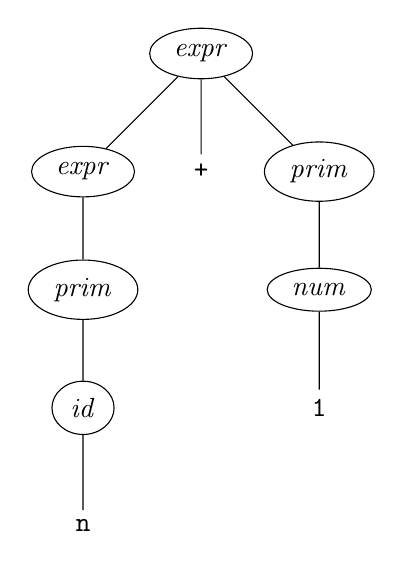
\begin{tikzpicture}
        \node[ellipse, draw] {\textit{expr}} 
        child {
            node[ellipse, draw] {\textit{expr}}
            child {
                node[ellipse, draw] {\textit{prim}}
                child {
                    node[ellipse, draw] {\textit{id}}
                    child {
                        node {\texttt{n}}
                    }
                }
            }
        }
        child {
            node {\texttt{+}}
        }
        child {
            node[ellipse, draw] {\textit{prim}}
            child {
                node[ellipse, draw] {\textit{num}}
                child {
                    node {\texttt{1}}
                }
            }
        };
    \end{tikzpicture}
    \caption{The syntax tree for the expression \texttt{n + 1}}
\end{figure}
\noindent The following is the syntax tree for the command \texttt{put n \textbackslash n}.
\begin{figure}[H]
    \centering
    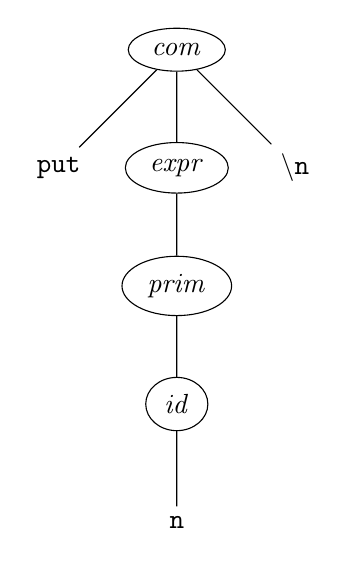
\begin{tikzpicture}
        \node[ellipse, draw] {\textit{com}}
        child {
            node {\texttt{put}}
        }
        child {
            node[ellipse, draw] {\textit{expr}}
            child {
                node[ellipse, draw] {\textit{prim}}
                child {
                    node[ellipse, draw] {\textit{id}}
                    child {
                        node {\texttt{n}}
                    }
                }
            }
        }
        child {
            node {\texttt{\textbackslash n}}
        };
    \end{tikzpicture}
    \caption{The syntax tree for the command \texttt{put n \textbackslash n}}
\end{figure}

Formally, for a grammar $G$, the syntax tree of $G$ is a tree where:
\begin{itemize}
    \item every terminal node is labelled by a terminal symbol of $G$.
    \item every non-terminal node is labelled by a non-terminal symbol of $G$.
    \item a non-terminal node labelled $N$ has children labelled $X$, $Y$, $Z$ (from left to right) if and only if $G$ has a product rule $N = XYZ$ or $N = \dots | XYZ | \dots$
\end{itemize}

\subsection{Language}
If $N$ is a non-terminal symbol of $G$, a phrase of class $N$ is a string of terminal symbols labelled the terminal symbols labelling the terminal nodes of a syntax whose root node is labelled $N$. We visit the terminal nodes from left to right. In Calc, some phrases are:
\begin{itemize}
    \item \texttt{x * (22 - y)}, a phrase of class \textit{expr};
    \item \texttt{set n = 42 \textbackslash n}, a phrase of class \textit{com};
    \item \texttt{set n = 42 \textbackslash n put x * (22 - y) \textbackslash n}, a phrase of class \textit{prog}.
\end{itemize}
If $S$ is the sentence symbol of $G$, a sentence of $G$ is a phrase of class $S$. In Calc, a phrase of class \textit{prog} is a sentence. Finally, the language generated by $G$ is the set of all sentences of $G$.

Our definition of language is syntax-driven since it is defined as a set of sentences. We are also interested in the semantics (i.e. the meaning of each sentence). A grammar does more than generate a set of sentences. It also imposes a phrase structure on each sentence, which we can see from the sentence's syntax tree. Once we know a sentence's phrase structure, we can use it to give a meaning to that sentence. 

For example, consider the extract of grammar below:
\begin{align*}
    \textit{expr} =&  \textit{ expr} \text{ `}\texttt{+}\text{' } \textit{prim} \\
    |\hspace{2pt} & \textit{ expr} \text{ `}\texttt{-}\text{' } \textit{prim} \\
    |\hspace{2pt} & \textit{ expr} \text{ `}\texttt{*}\text{' } \textit{prim}
\end{align*}
\noindent In this grammar, the operators \texttt{+}, \texttt{-} and \texttt{*} have the same precendence, as we can see in the syntax tree below.
\begin{figure}[H]
    \centering
    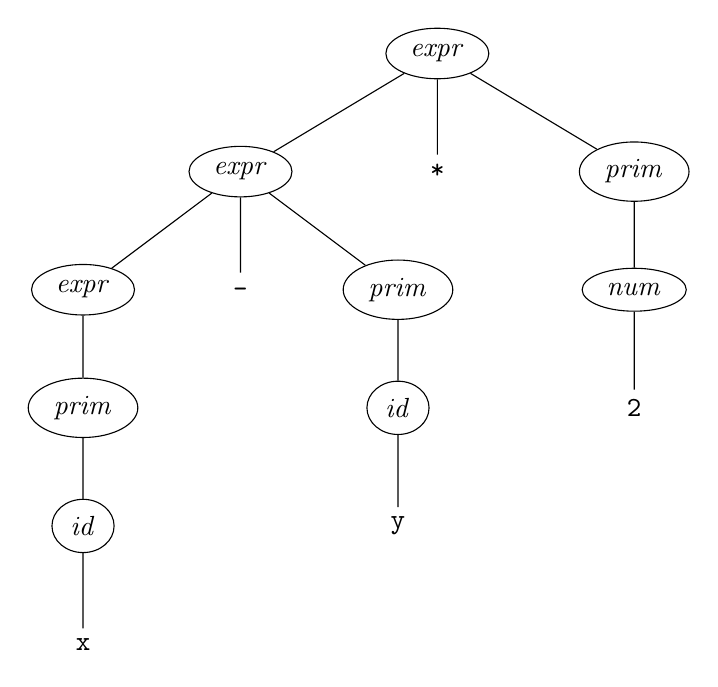
\begin{tikzpicture}[
        level 1/.style={sibling distance=2.5cm},
        level 2/.style={sibling distance=2cm},
        level 3/.style={sibling distance=1cm}
    ]
        \node[ellipse, draw] {\textit{expr}}
        child {
            node[ellipse, draw] {\textit{expr}}
            child {
                node[ellipse, draw] {\textit{expr}}
                child {
                    node[ellipse, draw] {\textit{prim}}
                    child {
                        node[ellipse, draw] {\textit{id}}
                        child {
                            node {\texttt{x}}
                        }
                    }
                }
            }
            child {
                node {\texttt{-}}
            }
            child {
                node[ellipse, draw] {\textit{prim}}
                child {
                    node[ellipse, draw] {\textit{id}}
                    child {
                        node {\texttt{y}}
                    }
                }
            }
        }
        child {
            node {\texttt{*}}
        }
        child {
            node[ellipse, draw] {\textit{prim}}
            child {
                node[ellipse, draw] {\textit{num}}
                child {
                    node {\texttt{2}}
                }
            }
        };
    \end{tikzpicture}
    \caption{The syntax tree for \texttt{x - y * 2}}
\end{figure}
\noindent So, the result will be \texttt{(x - y) * 2}. This is because we have placed the 3 operations \texttt{-}, \texttt{*} and \texttt{+} at the same level, and the tree is created left to right (i.e. \textit{expr} `\texttt{+}' \textit{prim} not \textit{prim} `\texttt{+}' \textit{expr}).

% We can use brackets to control the evaluation, as we can see in the syntax tree below.

% \begin{figure}[H]
%     \centering
%     \begin{tikzpicture}[
%         level 1/.style={sibling distance=2.5cm},
%         level 2/.style={sibling distance=2cm},
%         level 3/.style={sibling distance=1cm}
%     ]
%     \node[ellipse, draw] {\textit{expr}}
%         child {
%             node[ellipse, draw] {\textit{expr}}
%             child {
%                 node[ellipse, draw] {\textit{prim}}
%                 child {
%                     node[ellipse, draw] {\textit{id}}
%                     child {
%                         node {\texttt{x}}
%                     }
%                 }
%             }
%         }
%         child {
%             node {\texttt{-}}
%         }
%         child {
%             node[ellipse, draw] {\textit{prim}}
%             child {
%                 node {\texttt{(}}
%             }
%             child {
%                 node[ellipse, draw] {\textit{expr}}
%                 child {
%                     node[ellipse, draw] {\textit{expr}}
%                     child {
%                         node[ellipse, draw] {\textit{prim}}
%                         child {
%                             node[ellipse, draw] {\textit{id}}
%                             child {
%                                 node {\texttt{y}}
%                             }
%                         }
%                     }
%                 }
%                 child {
%                     node {\texttt{*}}
%                 }
%                 child {
%                     node[ellipse, draw] {\textit{prim}}
%                     child {
%                         node[ellipse, draw] {\textit{num}}
%                         child {
%                             node {\texttt{2}}
%                         }
%                     }
%                 }
%             }
%             child {
%                 node {\texttt{)}}
%             }
%         };
%     \end{tikzpicture}
%     \caption{The syntax tree for \texttt{x - (y * 2)}}
% \end{figure}

Now, consider the following grammar:
\begin{align*}
    \textit{expr} =& \textit{  term} \\
    |\hspace{2pt} & \textit{ expr } \text{`}\texttt{+}\text{'} \textit{ term} \\
    |\hspace{2pt} & \textit{ expr } \text{`}\texttt{-}\text{'} \textit{ term} \\
    \textit{term} =& \textit{ term } \text{`}\texttt{*}\text{'} \textit{ prim} 
\end{align*}
\noindent Within this grammar, we have a higher precedence for \texttt{*} than \texttt{+} and \texttt{-}. This can be seen in the syntax tree below.
\begin{figure}[H]
    \centering
    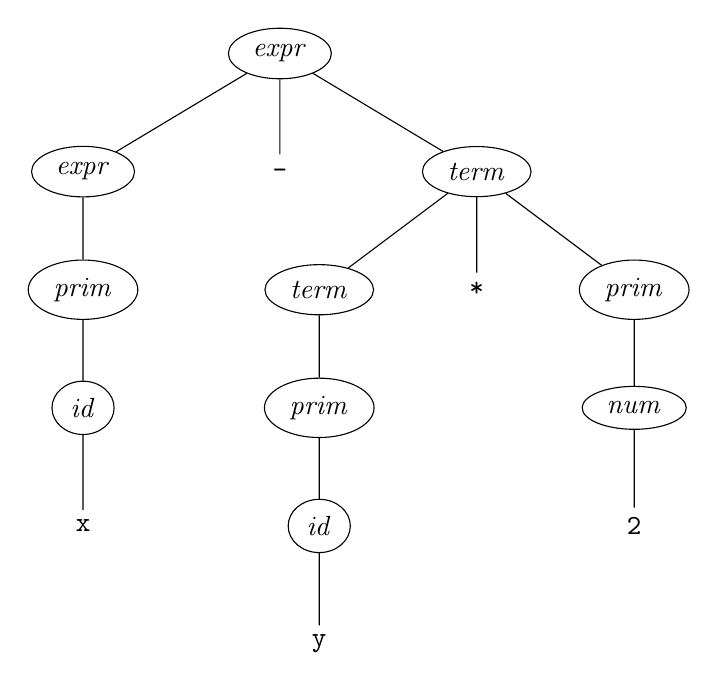
\begin{tikzpicture}[
        level 1/.style={sibling distance=2.5cm},
        level 2/.style={sibling distance=2cm},
        level 3/.style={sibling distance=1cm}
    ]
    \node[ellipse, draw] {\textit{expr}}
        child {
            node[ellipse, draw] {\textit{expr}}
            child {
                node[ellipse, draw] {\textit{prim}}
                child {
                    node[ellipse, draw] {\textit{id}}
                    child {
                        node {\texttt{x}}
                    }
                }
            }
        }
        child {
            node {\texttt{-}}
        }
        child {
            node[ellipse, draw] {\textit{term}}
            child {
                node[ellipse, draw] {\textit{term}}
                child {
                    node[ellipse, draw] {\textit{prim}}
                    child {
                        node[ellipse, draw] {\textit{id}}
                        child {
                            node {\texttt{y}}
                        }
                    }
                }
            }
            child {
                node {\texttt{*}}
            }
            child {
                node[ellipse, draw] {\textit{prim}}
                child {
                    node[ellipse, draw] {\textit{num}}
                    child {
                        node {\texttt{2}}
                    }
                }
            }
        };
    \end{tikzpicture}
    \caption{The syntax tree for \texttt{x - y * 2}}
\end{figure}
% \noindent This follows the rules of arithmetic, and we see this grammar in most PLs.

\subsection{Ambiguity}
A phrase is ambiguous if it has more than one syntax tree. Moreover, we say that a grammar is ambiguous if any of its phrases is ambiguous. 

Consider the following extract of a grammar.
\begin{align*}
    \textit{com} =& \text{ `}\texttt{if}\text{' } \textit{expr} \text{ `}\texttt{then}\text{' } \textit{com} \\
    |\hspace{2pt} & \text{ `}\texttt{if}\text{' } \textit{expr} \text{ `}\texttt{then}\text{' } \textit{com} \text{ `}\texttt{else}\text{' } \textit{com}
\end{align*}
\noindent We have 2 production rules for \texttt{if} where one syntax is a subpart of the other. This makes the grammar ambiguous. In particular, the phrase \texttt{if b then if c then put 1 else put 2} has two syntax trees, as shown below.
\begin{figure}[H]
    \centering
    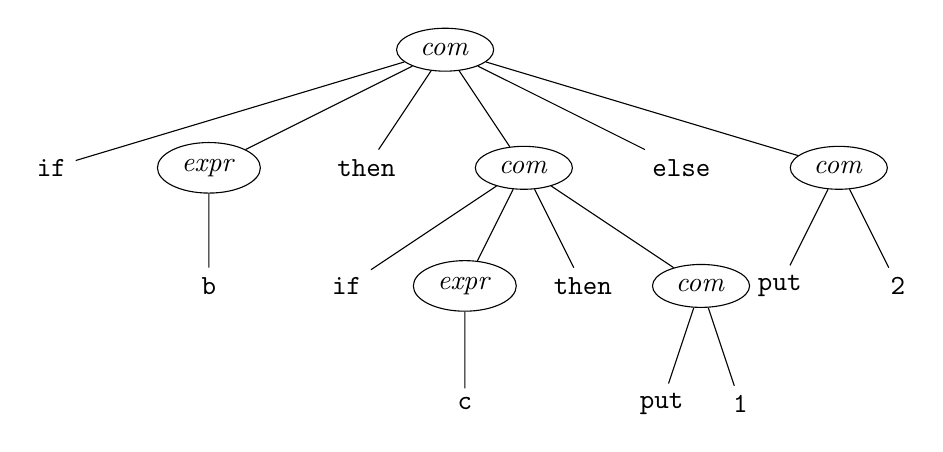
\begin{tikzpicture}[
        level 1/.style={sibling distance=2cm},
        level 2/.style={sibling distance=1.5cm},
        level 3/.style={sibling distance=1cm}
    ]
        \node[ellipse, draw] {\textit{com}}
        child {
            node {\texttt{if}}
        }
        child {
            node[ellipse, draw] {\textit{expr}}
            child {
                node {\texttt{b}}
            }
        }
        child {
            node {\texttt{then}}
        }
        child {
            node[ellipse, draw] {\textit{com}}
            child {
                node {\texttt{if}}
            }
            child {
                node[ellipse, draw] {\textit{expr}}
                child {
                    node {\texttt{c}}
                }
            }
            child {
                node {\texttt{then}}
            }
            child {
                node[ellipse, draw] {\textit{com}}
                child {
                    node {\texttt{put}}
                }
                child {
                    node {\texttt{1}}
                }
            }
        }
        child {
            node {\texttt{else}}
        }
        child {
            node[ellipse, draw] {\textit{com}}
            child {
                node {\texttt{put}}
            }
            child {
                node {\texttt{2}}
            }
        };
    \end{tikzpicture}
    \caption{A syntax tree for \texttt{if b then if c then put 1 else put 2}}
\end{figure}
\begin{figure}[H]
    \centering
    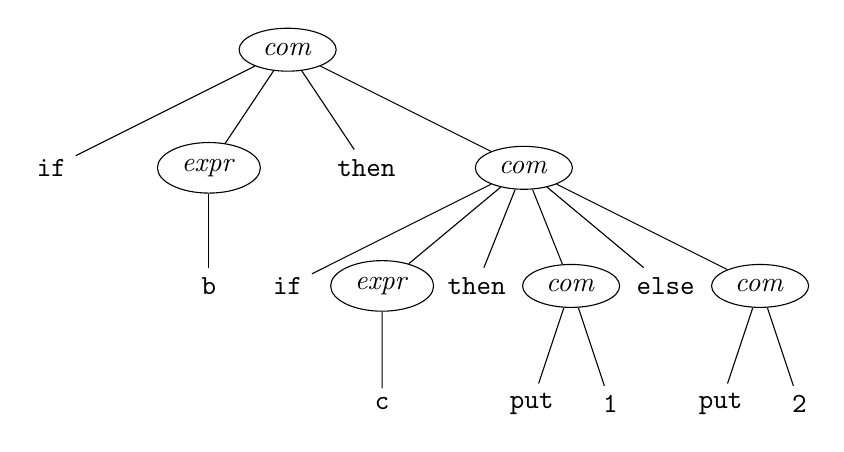
\begin{tikzpicture}[
        level 1/.style={sibling distance=2cm},
        level 2/.style={sibling distance=1.2cm},
        level 3/.style={sibling distance=1cm}
    ]
        \node[ellipse, draw] {\textit{com}}
        child {
            node {\texttt{if}}
        }
        child {
            node[ellipse, draw] {\textit{expr}}
            child {
                node {\texttt{b}}
            }
        }
        child {
            node {\texttt{then}}
        }
        child {
            node[ellipse, draw] {\textit{com}}
            child {
                node {\texttt{if}}
            }
            child {
                node[ellipse, draw] {\textit{expr}}
                child {
                    node {\texttt{c}}
                }
            }
            child {
                node {\texttt{then}}
            }
            child {
                node[ellipse, draw] {\textit{com}}
                child {
                    node {\texttt{put}}
                }
                child {
                    node {\texttt{1}}
                }
            }
            child {
                node {\texttt{else}}
            }
            child {
                node[ellipse, draw] {\textit{com}}
                child {
                    node {\texttt{put}}
                }
                child {
                    node {\texttt{2}}
                }
            }
        };
    \end{tikzpicture}
    \caption{A syntax tree for \texttt{if b then if c then put 1 else put 2}}
\end{figure}
We do not allow the grammar of a PL to be ambiguous so that the meaning of a program is certain.

\subsection{EBNF}
Extended Backus Naur Form (EBNF) is a combination of BNF and RE notation. An EBNF production rule has the form $N = \texttt{RE}$, where \texttt{RE} is a regular expression, expressed in terms of both terminal and non-terminal symbols. An example of such a rule is given below.
\[\textit{sequential-command } = \texttt{ \{ } \textit{command}^{\texttt{+}} \texttt{ \}}.\]
EBNF is convenient for specifying all aspects of syntax.

The EBNF production rules for Calc is given below:

\begin{figure}[H]
    \begin{align*}
        \textit{prog} =& \textit{ com}^{\texttt{*}}  \textit{ eof} \\
        \textit{com} =& \text{ `}\texttt{put}\text{' } \textit{expr eol} \\
        |\hspace{2pt} & \text{ `}\texttt{set}\text{' } \textit{id } \text{`}\texttt{=}\text{'} \textit{ expr eol} \\
        \textit{expr} =& \textit{  prim } (\text{`}\texttt{+}\text{'} \textit{ prim }|\text{ `}\texttt{-}\text{'} \textit{ prim }|\text{ `}\texttt{*}\text{'} \textit{ prim})^{\texttt{*}} \\
        \textit{prim} =& \textit{ num} \\
        |\hspace{2pt} & \textit{ id} \\
        |\hspace{2pt} & \text{ `}\texttt{(}\text{' } \textit{ expr } \text{ `}\texttt{)}\text{'} \\
        \textit{letter} =& \text{ `}\texttt{a}\text{' } | \text{ `}\texttt{b}\text{' } | \dots | \text{ `}\texttt{z}\text{' } \\
        \textit{digit} =& \text{ `}\texttt{0}\text{' } | \text{ `}\texttt{1}\text{' } | \dots | \text{ `}\texttt{9}\text{'} \\
        \textit{eol} =& \text{ `}\texttt{\textbackslash n}\text{'}
    \end{align*}
    \caption{The EBNF production rules for Calc.}
\end{figure}

\newpage

\section{Values and Types}
Values are grouped into types according to the operations that may be performed on them. Different PLs support a huge variety of types, such as integers, floats, booleans, characters, objects, etc. A type is a set of values equipped with operations that can be applied uniformly to all these values, e.g. the type \texttt{BOOL} has values $\{\texttt{true}, \texttt{false}\}$ with operations \texttt{not}, \texttt{and}, \texttt{or}. The cardinality of a type $T$ is the number of values of type $T$, and is denoted by $\#T$, e.g. $\#\texttt{BOOL} = 2$.

A value $v$ of type $T$ is an element $v \in T$. For example, the value \texttt{false} is of type \texttt{BOOL}, and the value \texttt{13} is of type \texttt{INT}. An expression $E$ is of type $T$ if its (expected) evaluation results in a value $v$ of type $T$. For example, if \texttt{n} is of type \texttt{INT}, then \texttt{n - 1} is an expression of type \texttt{INT}, and \texttt{n > 0} is an expression of type \texttt{BOOL}.

\subsection{Primitive types}
A primitive type is a type whose values are primitive. That is, they cannot be decomposed into smaller values. Every PL has many built-in primitive types. The choice of primitive types is influenced by the PL's intended application area, e.g.
\begin{itemize}
    \item Fortran (scientific computing) has floating point numbers,
    \item Cobol (data processing) has fixed-length strings,
    \item C (system programming) has bytes and pointers.
\end{itemize}
Some PLs allow programmers to define new primitive types.

Below are some common built-in primitive types:
\begin{align*}
    \texttt{VOID} &= \{\texttt{void}\} \\
    \texttt{BOOL} &= \{\texttt{true}, \texttt{false}\} \\
    \texttt{CHAR} &= \{\texttt{A}, \dots, \texttt{Z}, \dots \} \\
    \texttt{INT} &= \{\texttt{-m}, \dots, \texttt{-1}, \texttt{0}, \texttt{1}, \dots, \texttt{m-1}\} \\
    \texttt{FLOAT} &= \{\dots, \texttt{0.0}, \dots\}.
\end{align*}
The types \texttt{CHAR}, \texttt{INT} and \texttt{FLOAT} are present in most PLs, but there are some differences in their implementation depending on the PL/implementation. Now, we consider the cardinalities of the sets:
\begin{itemize}
    \item $\#\texttt{VOID} = 1$,
    \item $\#\texttt{BOOL} = 2$,
    \item $\#\texttt{CHAR} = 128, 256, 32768, \dots$ (depends on the language),
    \item $\#\texttt{INT} = 2m$.
\end{itemize}
The definition of primitive types depends on the PL, e.g. in C, booleans, characters and enums are just (small) numbers.

\subsection{Composite types}
A composite type is a type whose values are composite. This means that these values can be decomposed into simpler values. In a PL, there are 4 fundamental ways of generating composite types from primitive/composite types:
\begin{itemize}
    \item Cartesian products, which gives rise to tuples, structs and records;
    \item disjoint unions, which give algebraic types, variant records and objects;
    \item mappings, which give arrays and functions;
    \item recursive types, which give rise to lists and trees.
\end{itemize}

\subsubsection{Cartesian product}
In a Cartesian product, values of two (or more) types are grouped into pairs (or tuples). Formally, for types $S$ and $T$, the product type $S \times T$ has values of the form $(s, t)$, where $s$ is a value of type $S$ and $t$ is a value of type $t$. In other words,
\[S \times T = \{(s, t) \mid s \in S, t \in T\}.\]
The cardinality of the Cartesian product type is given by $\#(S \times T) = \#S \times \#T$. We can generalise from pairs to tuples:
\[S_1 \times \dots \times S_n = \{(s_1, \dots, s_n) \mid s_1 \in S_1, \dots, s_n \in S_n\}.\]

There are 2 basic operations we can perform on tuples:
\begin{itemize}
    \item we can construct a tuple given its components;
    \item we can select a specific component from a tuple.
\end{itemize}

Pascal records, C structs and Haskell tuples can all be understood in terms of cartesian products. Python tuples are somewhat different from normal tuples. This is because they can be indexed like arrays. The following shows the tuple operations on C structs:
\begin{lstlisting}[language=c]
enum Month {
    JAN, FEB, MAR, APR, MAY, JUN,
    JUL, AUG, SEP, OCT, NOV, DEC};
struct Date {Month m; int d;}

struct Date date1 = {JAN, 1};
printf ("%d/%d", date1.d, date1.m+1);
\end{lstlisting}
As an enumerated type, \texttt{Month} has values 0 to 11. We construct a struct by \texttt{\{JAN, 1\}}, and select the components by \texttt{date1.d} and \texttt{date1.m}. The possible values of struct type are 
\[\texttt{MONTH} \times \texttt{INT} = \{0, 1, \dots, 11\} \times \{\dots, -1, 0, 1, \dots\}.\]

\subsubsection{Disjoint union}
In a disjoint union, a value is chosen from one of two (or more) types. So, the union type $S + T$ is the type of disjoint-union values. Each disjoint-union value consists of a variant (chosen from either type $S$ or type $T$), along with a tag:
\[S + T = \{\texttt{left } s \mid x \in S\} \cup \{\texttt{right } t \mid t \in T\}.\]
The value \texttt{left} $s$ consists of the tag \texttt{left} and a variant $s \in S$. Similarly, the value \texttt{right} $t$ consists of the tag \texttt{right} and a variant $t \in T$. We can write $\texttt{left } S + \texttt{right } T$ to make the tags explicit. The cardinality of the disjoint union type $\#(S + T) = \#S + \#T$. We can generate to disjoint unions with multiple variants: $T_1 + T_2 + \dots + T_n$.

There are 3 basic operations we can perform on disjoint-union values:
\begin{itemize}
    \item construction of a disjoint-union value from its tag and variant;
    \item tag test, to inspect the tag of the disjoint-union value;
    \item projection, to recover a specific variant of a disjoint-union value (e.g. its $T_1$ variant). Trying to recover the wrong variant will fail.
\end{itemize}

Haskell algebraic types, Pascal/Ada variant records and Java objects can be understood in terms of disjoint unions. The following shows the disjoint-union operations on Java objects:
\begin{lstlisting}[language=java]
class Point {
    Point () {
        // code
    }
    // code
}

class Circle extends Point {
    int r;
    Circle (int r) {
        this.r = r;
    }
    // code
}

class Box extends Point {
    int w;
    int h;
    Box (int w, int h) {
        this.w = w;
        this.h = h;
    }
}
\end{lstlisting}
So, the set of objects in Java is:
\[\texttt{OBJECT} = \dots + \texttt{Point VOID} + \texttt{Circle INT} + \texttt{Box (INT} \times \texttt{INT)} + \dots\]
The other objects are library classes and the other declared classes. We have objects: \texttt{Point VOID}, \texttt{Circle 5}, \texttt{Box (3, 8)}, etc. Each object's tag identifies its class.

The operations we can perform on these Java classes are given below:
\begin{lstlisting}[language=java]
Circle c = new Circle(5);
Box b = new Box(3, 4);

Point p;
if (p instanceof Circle) {
    int radius = ((Circle) p).r;
    // code
}
\end{lstlisting}
We construct objects in lines 1 and 2. In line 5, we perform a tag test- \texttt{p instanceof Circle}. In line 5, we project a point into a circle- \texttt{(Circle) p}.

The set of objects in a Java program is open-ended. Initially, the set contains objects of library classes (non-abstract). Subsequently, the set is augmented by each declared class (non-abstract). We exclude abstract classes since it is not possible to instantiate those.

\subsubsection{Mapping types}
A map $m: S \to T$ maps a value in $S$ to a value in $T$. We denote $y = m(x)$, and call $y$ the image of $x$ under $m$. The set $S \to T$ is the type of all mappings $m: S \to T$.
\[S \to T = \{m \mid x \in S \implies m(x) \in T\}.\]
The cardinality of the mapping type $\#(S \to T) = (\#T)^S$. This is because, for each $s \in S$, there are $\# T$ possible choices for $m(s)$.

For example, consider the mapping type:
\[\{u, v\} \to \{a, b, c\}.\]
Its cardinality is 9, and the possible mappings are:
\begin{align*}
    & \{u \to a, v \to a\} && \{u \to a, v \to b\} && \{u \to a, v \to c\} \\
    & \{u \to b, v \to a\} && \{u \to b, v \to b\} && \{u \to b, v \to c\} \\
    & \{u \to c, v \to a\} && \{u \to c, v \to b\} && \{u \to c, v \to c\}.
\end{align*}

Arrays can be understood as mappings. Assume that we have an array with components of type $T$ and index values of type $S$. Then, for every possible index in $S$, there exists a component $t$ of type $T$. This gives a natural representation of the array as the mapping type $S \to T$. The basic operations we can do on arrays are:
\begin{itemize}
    \item construction of an array from its components; and
    \item indexing, to select a component using a computed index value.
\end{itemize}

An array is a finite mapping. If an array is of type $S \to T$, $S$ must be a finite range of consecutive values (starting from a lower bound and going to the upper bound, incrementing by 1 every time), called the array's index range. In some PLs, the index may be any range of integers. However, the index range is mostly $\{0, 1, \dots, n-1\}$, for some fixed $n$.

We now consider C arrays:
\begin{lstlisting}[language=C]
enum Pixel {DARK, LIGHT};
typedef Pixel[] Row;

Row r = {DARK, LIGHT, LIGHT, DARK}
int i, j;
r[i] = r[j];
\end{lstlisting}
We construct the array \texttt{r} in line 4, and index \texttt{r[j]} in line 6.
The values of this array type are: 
\[\texttt{ROW} = \{0, 1, 2, \dots\} \to \texttt{PIXEL} = \{0, 1, 2, \dots, \} \to \{0, 1\}.\]

Functions can also be understood as mappings. They map arguments to results. For example, let $f$ be a unary function whose argument is of type $S$ and result is of type $T$. Then, $f$ is of type $S \to T$. There are 2 operations on functions:
\begin{itemize}
    \item construction (or definition) of a function.
    \item application, i.e. calling the function with an argument.
\end{itemize}
A function can represent an infinite mapping (if $\# S = \infty$). This is not an issue since the results are computed on demand. On the other hand, this is an issue for an array since all the components within the array are stored.

A binary function $f$ has arguments of type $S_1$ and $S_2$, and result of type $T$. In most PLs, we view $f$ as mapping a single pair of arguments (i.e. $S_1 \times S_2$) to a result. So, the function is of the form $f: (S_1 \times S_2) \to T$. Then, we can think of $f$ as a unary function. This can be generalised to $n$-ary functions, i.e. $f: (S_1 \times \dots \times S_n) \to T$.

Now, consider the following unary function in C:
\begin{lstlisting}[language=C]
int length (String s) {
    int n = 0;
    while (s[n] != NUL) {
        n++;
    }
    return n;
}
\end{lstlisting}
This function's type is $\texttt{STRING} \to \texttt{INT}$. The value of the function is an infinite mapping since there are infinite possible strings. Next, consider the following binary function in C:
\begin{lstlisting}[language=C]
String rep (int n, char c) {
    String s = malloc((n+1) * sizeof(char));
    for (int i = 0; i < n; i++) {
        s[i] = c;
    }
    s[n] = NUL;
    return s;
}
\end{lstlisting}
This function has type $(\texttt{INT} \times \texttt{CHAR}) \to \texttt{STRING}$. In a call, the function is applied to a pair, e.g. $(\texttt{6}, \texttt{!})$ yields \texttt{!!!!!!}.

\subsection{Recursive types}
A recursive type is one defined in terms of itself. It must be a disjoint-union type in which:
\begin{itemize}
    \item at least one variant is recursive (the recursive type) and
    \item at least one variant is non-recursive (the base type).
\end{itemize}
The types \texttt{LIST} and \texttt{TREE} can be given as recursive types:
\[\texttt{LIST} = \texttt{VOID} + (\texttt{VALUE} \times \texttt{LIST}), \qquad \texttt{TREE} = \texttt{VOID} + (\texttt{VALUE} \times \texttt{TREE} \times \texttt{TREE}).\]
The cardinality of a recursive type $T$ is always infinite, i.e. $\# T = \infty$. We can produce a value of type $T$ for an arbitrarily large size by taking higher numbers of the recursive case.

A list is a sequence of 0 or more component values. It can be empty or non-empty. If it is not empty, then it can be thought of as containing a head (the first value), and a tail (everything else in the list, as another list). This leads to the recursive relation
\[\texttt{LIST} = \texttt{empty VOID} + \texttt{nonempty } (\texttt{VALUE} \times \texttt{LIST}).\]

For example, consider the following class declaration for integer lists in Java:
\begin{lstlisting}[language=java]
class IntList {
    int head;
    IntList tail;
}
\end{lstlisting}
The non-recursive variant is the built-in \texttt{null} value.

A string is a sequence of 0 or more characters. The way they are treated depends on the PL:
\begin{itemize}
    \item Python treats strings as primitive.
    \item Haskell treats strings as lists of characters, which gives them all the list operations (e.g. getting the head and the tail).
    \item C treats strings as an array of characters, which gives them all the array operations (e.g. indexing).
    \item Java treats strings as objects of class \texttt{String}.
\end{itemize}

\subsection{Type systems}
A type error occurs when a program performs a meaningless operation, e.g. adding a string to a boolean. A PL's type system groups values into types to help prevent type errors. It also allows programmers to describe data effectively. Possession of a type system distinguishes high-level PLs from low-level languages. In assembly/machine languages, the only `types' are bytes, so meaningless operations cannot be prevented.

Before any operation is performed, its operands must be type-checked in order to prevent a type error. For example,
\begin{itemize}
    \item in a not operation, we must check that the operand is a boolean;
    \item in an add operation, we must check that both operands are numbers;
    \item in an indexing operation, we must check that the left operand is an array and the right operand is an integer.
\end{itemize}

We can classify a PL with respect to its type system. There are 2 types of type systems- static and dynamic typing. In a statically typed PL:
\begin{itemize}
    \item every variable has a fixed type (which is usually described by the programmer), 
    \item every expression has a fixed type (which is usually inferred by the compiler), and
    \item all operands are type-checked at compile-time.
\end{itemize}
Some statically typed languages are: Pascal, Ada, C, Java and Haskell. On the other hand, in a dynamically typed PL:
\begin{itemize}
    \item only values have fixed types,
    \item variables and expressions do not have fixed types, and
    \item operands must be type-checked when they are computed at run-time.
\end{itemize}
Some dynamically typed languages are: Smalltalk, Lisp, Prolog and (most) scripting languages such as Perl and Python.

Consider the following code in Java:
\begin{lstlisting}[language=java]
public static boolean even (int n) {
    return n % 2 == 0;
}

public static void main(String[] args) {
    int p;
    if (even(p+1)) {
        // code
    } else {
        // code
    }
}
\end{lstlisting}
When compiling lines 1-3, the compiler doesn't know the value of \texttt{n}, but does know that its type is \texttt{INT}. Using this information, it knows that the expression in line 2 will be a \texttt{BOOL}. Similarly, in line 7, the compiler does not know the value of \texttt{p+1}, but it does know that its type is \texttt{INT}. This matches the parameter type for the function \texttt{even}, so does not cause a type error. Clearly, we do not need to know the values of the variables to ensure that there won't be any type errors at runtime.

Now, consider the same code in Python:
\begin{lstlisting}[language=python]
def even(n):
    return n % 2 == 0
\end{lstlisting}
Here, the type of the variable \texttt{n} is not known. So, the operation \texttt{\%} must be protected by a run-time type check. This is because we do not declare the types of variables in Python, so the compiler cannot infer them in general. So, we need run-time type checks to detect type errors.

Using a dynamically typed language, we can make use of the same function declaration for different types. To see this, consider the following code in Python.
\begin{lstlisting}[language=python]
# Return the minimum element of values
def minimum(values):
    min_val = values[0]
    for val in values:
        if val < min_val:
            min_val = val
    return min_val
\end{lstlisting}
Here, the parameter \texttt{value} can be a list, or tuple, and its components can be string, int or float. So, we can call the function \texttt{minimum} with the tuple \texttt{(3.0, 2.7, 4.1)}, list of integers \texttt{[2, 3, 5, 7]} or a list of string \texttt{[cat, dog, ant]}.

There are advantages and disadvantages to both static and dynamic typing:
\begin{itemize}
    \item Static typing is more efficient. It only requires compile-time type checks. On the other hand, dynamic typing requires run-time type checks, which makes the program run slower. Moreover, we also need to tag all the values, which uses more space.
    \item Static typing is more secure. The compiler can guarantee that the object program contains no type errors. Dynamic typing provides no such security.
    \item Static typing is less flexible. Certain computations cannot be expressed naturally. Dynamic typing is more natural when processing data whose types are not known at compile-time.
\end{itemize}

\subsection{Expressions}
An expression is a program construct that can be evaluated to yield a value. Simple expressions are literals and variables. Compound expressions are given below:
\begin{itemize}
    \item A function call is an expression that computes a result by applying a function to argument(s).
    \item A construction is an expression that constructs a composite value from its components.
    \item A conditional expression is an expression that chooses one of its sub-expressions to evaluate.
    \item An iterative expression is an expression that performs a computation over a collection (e.g. an array or a list).
    \item A block expression is an expression that contains declarations of local variables.
\end{itemize}

\end{document}
